\subsection*{Sprint 3: Pantalla de inicio y controles de calidad del texto}
\addcontentsline{toc}{subsection}{Sprint 3: Pantalla de inicio y controles de calidad del texto}

El tercer sprint se centra en el diseño y desarrollo de la \textbf{pantalla de
	inicio} de la aplicación \textbf{Muncher}. Aunque pueda parecer una tarea
limitada en alcance, este hito marca el inicio de la construcción del front‑end
y sienta las bases de la identidad visual y de la experiencia de usuario del
sistema. Su implementación implica definir la estructura fundamental de la
interfaz y establecer criterios visuales y técnicos que guiarán el desarrollo
de las siguientes vistas.

Durante este sprint se tomarán decisiones clave sobre la arquitectura del
front‑end, como la elección entre utilizar una librería de componentes
preexistente de React —por ejemplo, MUI o Chakra UI— o desarrollar un conjunto
propio de componentes adaptados a las necesidades del proyecto. Además, se
trabajará en la definición de la identidad visual, seleccionando la paleta de
colores, tipografías y elementos gráficos que representarán la marca
\textbf{Muncher} en todas las pantallas.

Otro aspecto esencial será garantizar un diseño \textbf{responsivo}, capaz de
adaptarse correctamente a diferentes tamaños de pantalla y dispositivos. Esto
implicará definir un sistema de maquetación flexible y patrones de diseño
reutilizables que aseguren coherencia visual y una experiencia fluida tanto en
escritorio como en dispositivos móviles. En resumen, este sprint establecerá
los cimientos visuales y técnicos sobre los que se construirá toda la interfaz
de usuario de la aplicación.

La pantalla de inicio deberá incluir una serie de elementos clave orientados a
la comunicación y a la usabilidad. Se incorporará una \textbf{barra de
	navegación} que permita acceder a las principales secciones de la aplicación, y
un \textbf{llamado a la acción} (\textit{call to action}) destacando las
opciones para registrarse o iniciar sesión. Asimismo, se diseñará una
\textbf{hero section} que muestre de manera clara y atractiva la utilidad y el
valor principal de \textbf{Muncher} desde el primer vistazo. Finalmente, se
añadirá una \textbf{lista de recetas destacadas} visible incluso sin iniciar
sesión, de modo que los nuevos usuarios puedan explorar parte del contenido y
comprender el propósito de la aplicación antes de registrarse.

\subsubsection*{Objetivos iniciales}

\begin{itemize}
	\item Seleccionar el enfoque a la hora de crear los componentes del front-end:
	      librería de componentes preexistente o desarrollo propio.
	\item Seleccionar un sistema de gestión de estilos: CSS puro, CSS Modules, CSS in JS
	      o Tailwind CSS.
	\item Definir la paleta de colores, tipografías y elementos gráficos que
	      representarán la marca \textbf{Muncher} en todas las pantallas.
	\item Maquetar la pantalla de inicio de forma responsiva y accesible.
	\item Implementar la pantalla de inicio en el front-end.
	\item Asegurarse de que los textos de la aplicación se almacenan de forma separada al
	      código.
	\item Añadir control de ortografía y gramática a los textos de la aplicación.
\end{itemize}

\subsubsection*{Historias de usuario completadas}

\begin{center}
	\begin{tabularx}{\textwidth}{|l|X|c|}
		\hline
		\textbf{Identificador} & \textbf{Nombre}                      & \textbf{Puntos de historia} \\
		\hline
		\usref{US-MF-01}       & Maquetación de la pantalla de inicio & 5                           \\
		\hline
		\usref{US-MF-02}       & Internacionalización                 & 3                           \\
		\hline
		\usref{US-CI-05}       & Control de ortografía y gramática    & 2                           \\
		\hline
	\end{tabularx}
\end{center}

\subsubsection*{Retrospectiva}

El tercer sprint ha concluido con la definición de la identidad visual de
\textbf{Muncher} y la implementación funcional de su interfaz de bienvenida. El
proceso de toma de decisiones técnicas ha sido fundamental para equilibrar la
personalización estética con la eficiencia en el desarrollo.

En cuanto a la arquitectura de componentes, se ha optado por un
\textbf{desarrollo propio} en lugar de depender de librerías de componentes
cerradas como MUI o Chakra UI. Esta decisión se fundamenta en la búsqueda de la
máxima flexibilidad y en la disponibilidad de recursos y documentación actual
que simplifican la creación de componentes a medida. El uso de referencias como
\textbf{Flowbite} ha permitido adoptar un enfoque "hecho a mano" pero altamente
eficiente, obteniendo componentes totalmente funcionales y adaptados a las
necesidades específicas del proyecto sin la sobrecarga de una librería externa.

Para la gestión de estilos, se ha seleccionado \textbf{Tailwind CSS}. Su
facilidad de configuración, el impacto mínimo en el tamaño del \textit{bundle}
final y la agilidad que ofrece para la creación de temas dinámicos fueron los
factores determinantes frente a alternativas como CSS puro o CSS-in-JS.

A nivel de diseño, se ha definido una identidad visual disruptiva: un estilo
\textbf{desenfadado, colorido y divertido} inspirado en la estética de las
revistas juveniles de los años 80 y 90. Esta dirección artística se materializa
en una paleta de colores vibrante, el uso de formas angulosas con sombras muy
marcadas y una tipografía de estilo urbano o \textit{grunge} para los
titulares, dotando a la aplicación de una personalidad única en su sector.

Finalmente, la maquetación se ha ejecutado bajo un enfoque
\textbf{\textit{mobile-first}}. Este flujo de trabajo ha garantizado que la
experiencia de usuario sea óptima en dispositivos móviles desde el inicio,
facilitando la adaptación progresiva de la interfaz a pantallas de mayor
resolución mediante los \textit{breakpoints} nativos de Tailwind, asegurando
así una responsividad total y una jerarquía visual coherente en todo momento.

Por otro lado, se ha implementado la infraestructura para la
\textbf{internacionalización (i18n)} de la aplicación. Aunque actualmente el
sistema se ofrece exclusivamente en español, se ha considerado crítico ejecutar
esta tarea en las etapas iniciales del desarrollo. Integrar un sistema de
traducción una vez que la interfaz está avanzada supondría una refactorización
titánica para extraer cientos de cadenas de texto embebidas en el código. Al
centralizar todos los literales en ficheros de configuración independientes
(habitualmente en formato \texttt{JSON}), se facilita no solo la futura
escalabilidad a otros idiomas, sino también el mantenimiento y la consistencia
editorial del sitio.

Esta separación de intereses entre la lógica de presentación y el contenido
textual ofrece una ventaja adicional: la optimización de los flujos de
\textbf{control de calidad}. Al residir los textos fuera del código fuente, es
posible aplicar herramientas automáticas de control de ortografía y gramática
de manera mucho más sencilla y eficiente. Esto garantiza que la comunicación
con el usuario final mantenga un estándar de calidad profesional, minimizando
errores tipográficos que podrían pasar desapercibidos en una revisión manual
del código.

Finalmente, para materializar este control de calidad sobre los textos
extraídos, se ha integrado \textbf{cspell} como herramienta de corrección
ortográfica. La elección de esta utilidad frente a otras alternativas como
\textit{typos} —más orientada al ecosistema anglosajón— se debe a su robusto
soporte y amplio diccionario para el idioma \textbf{español}. Además, su
capacidad de integración directa con \textbf{ESLint} ha permitido unificar la
validación de la sintaxis del código y la corrección tipográfica bajo un mismo
flujo de ejecución. De este modo, mediante un único comando, el sistema es
capaz de detectar tanto errores de programación como erratas en los contenidos
de la interfaz, garantizando una entrega de software pulida en todos sus
aspectos.

\vspace{1cm}

\begin{figure}[H]

	\begin{subfigure}{0.5\textwidth}
		\centering
		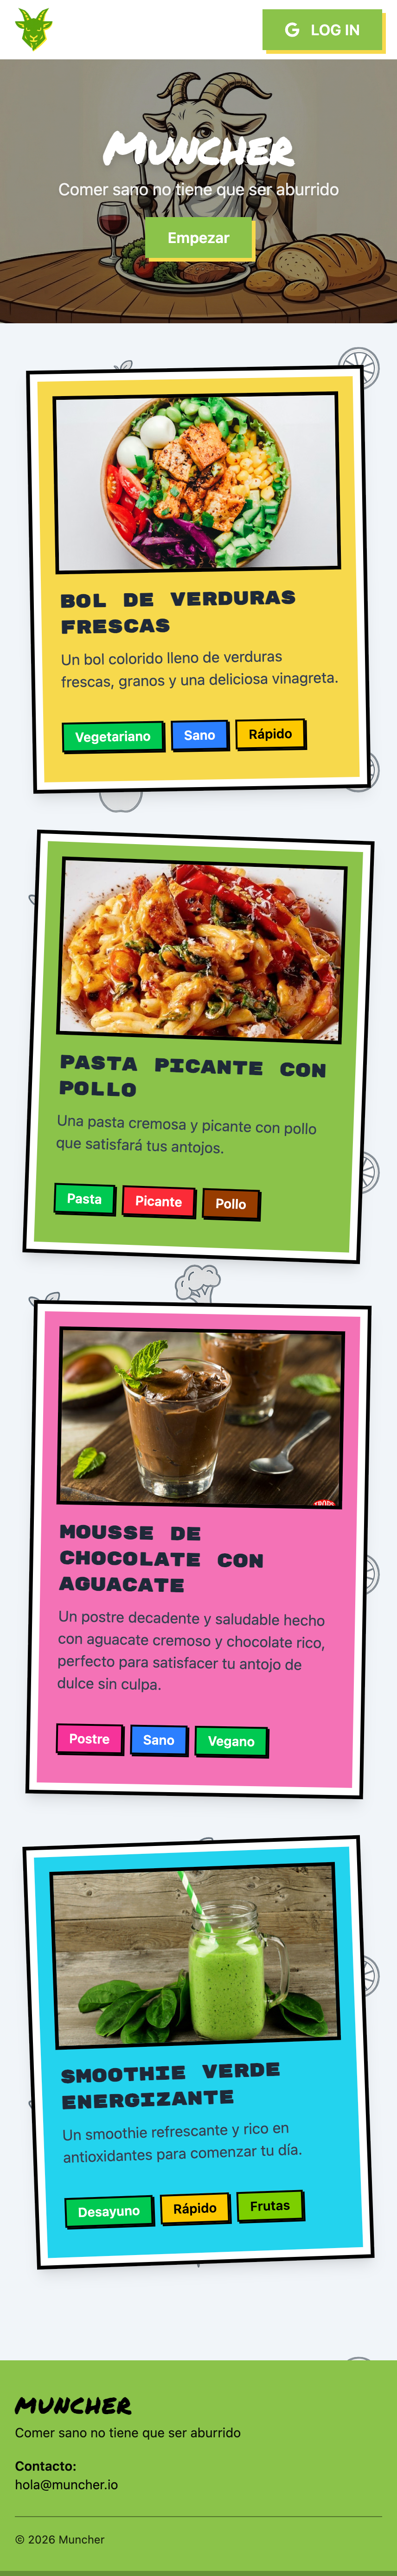
\includegraphics[height=12cm]{../img/mobile-home-page.png}
		\caption{Diseño para móviles}
		\label{fig:sub-design-home-page-mobile}
	\end{subfigure}
	\begin{subfigure}{0.5\textwidth}
		\centering
		\includegraphics[height=12cm]{../img/desktop-home-page.png}
		\caption{Diseño para ordenadores}
		\label{fig:sub-design-home-page-desktop}
	\end{subfigure}

	\caption{Diseño de la pantalla de inicio de \textbf{Muncher} para dispositivos móviles y ordenadores.}
	\label{fig:design-home-page}
\end{figure}
